\section{Discussion}
\label{sect:prob-discussion}

We discuss potential applications, extensions, and connections of probabilistic property evaluation in the following.

\subsection{Probabilistic equivalence checking}
\begin{figure}[t]
    \centering
    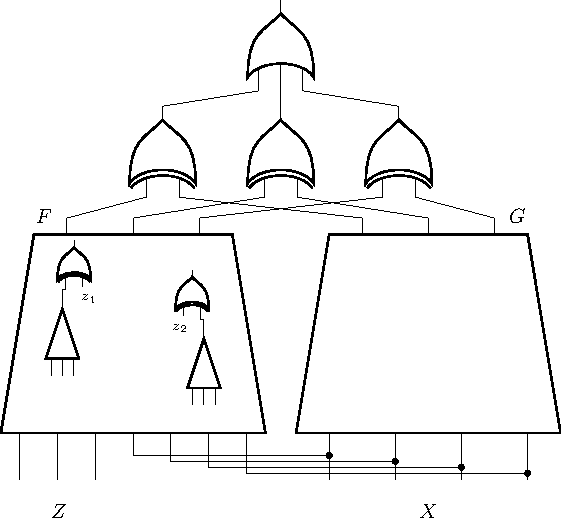
\includegraphics{fig/build/pec-miter.pdf}
    \caption{A miter SPBN for probabilistic equivalence checking}
    \label{fig:prob-PEC}
\end{figure}
Given two SPBNs, their equivalence checking can be easily formulated under PPE and MPPE framework,
as depicted in~\cref{fig:prob-PEC}.
The property network corresponds to a miter circuit
that tests the difference of corresponding outputs of the two SPBNs,
same as in the equivalence checking of deterministic designs.
With the proposed framework,
we can analyze the average (resp. maximum) probability
that the two SPBNs are functionally different through PPE (resp. MPPE).
We refer to the equivalence checking problem as
\textit{probabilistic equivalence checking} (PEC) for the average-case analysis and
\textit{maximum probabilistic equivalence checking} (MPEC) for the worst-case analysis.
Since equivalence checking is widely encountered,
our experiments will focus on PEC and MPEC to compare the strengths and weaknesses of different solutions
that we proposed in~\cref{sect:prob-solutions}.

\subsection{Prioritized output requirement}
For some applications,
we may want to impose different criticality requirements on different output signals.
Given an SPBN $G$ over
primary inputs $X$,
internal vertices $Y$,
and auxiliary inputs $Z$,
this output-prioritized version of MPPE is naturally expressible
in terms of stochastic integer linear programming (SILP)~\cite{Schultz2003} as follows:
\begin{align*}
    \max_X \enskip \mathbb{E}[\sum_{i=1}^n w_i o_i(X,Y,Z)] \enskip s.t. \enskip \pf,
\end{align*}
where $o_i \in V_O$ is an output of $G$, $|V_O|=n$,
$w_i$ is the weight of $o_i$,
$\mathbb{E}[\cdot]$ denotes the expectation value,
and $\pf$ is a set of linear inequalities derived from the CNF formula of $G$
through the standard translation from clauses to linear constraints.
To illustrate, a clause $(x \lor \lnot y \lor z)$ in a CNF formula is transformed into
a linear inequality $(x+1-y+z)\geq 1$,
or $(x-y+z)\geq 0$ in $\pf$.
Note that the worst case formulation in~\cref{thm:prob-mppe-ssat} is a special case of
the SILP formulation where the expectation value of the miter's output is maximized.

\subsection{Connection to approximate design analysis}
Approximate design analysis assesses the deviation between
an approximate design and its exact counterpart in two scenarios:
the worse and average cases.
For the worst-case analysis, integer linear programming (ILP) can be applied
to find an input assignment to maximize the number of deviating outputs.
For the average-case analysis, model counting can be used
to compute the number of input assignments that make the two designs have different output responses.
In both cases, our PPE framework can be applied to analyze an approximate design,
which can be seen as a probabilistic design without random behavior.
For probabilistic design analysis,
if all random variables become deterministic,
then it degenerates to approximate design analysis
(from SILP to ILP under the worst-case analysis and
from weighted model counting to model counting under the average-case analysis).